%%%%%%%%%%%%%%%%%%%%%%%%%%%%%%%%%%%%%%%%%%%%%%%%%%%%%%%%%%%%%%%%%%%%%%%%%%%%%%%%
%  Policy Evaluation Lab -- Lecture 9: The new EU economic governance and the
%  ECB. Thursday 19 November 2026.
%  Slides on the 2024 rules and Italy reuse the special-session slides of
%  23 Oct 2026 (never taught), already checked line by line
%  (materials/readings/special-session-budget/CLAIMS-CHECK.md).
%  New sources, checked 18 Nov 2026 (stored in materials/readings/part-2/ and
%  slides-src/sources/lecture-09/):
%   - Council Recommendation activating Italy's national escape clause,
%     ST 14668/26 (3 Nov 2026) and COR 1 REV 3 (13 Nov 2026): request of
%     11 Sept 2026; defence 1.3% of GDP 2024-2026 (Table 1); up to +0.9 pp
%     defence by end-2028; total deviation cap 1.5% of GDP; energy 0.3%/yr,
%     0.6% cumulative, 2026-2028; full use => 2028 deficit +1.1 pp, debt
%     +1.3 pp; energy measures "targeted and cost-effective"; reporting twice a
%     year (15 April, 15 October) with "evidence regarding their eligibility";
%     deviations not recorded in the control account.
%   - MEF press release, 9 Nov 2026: approved at Ecofin; budget law 2027 uses
%     up to 0.3% of GDP for defence and 0.3% for energy in 2027 and 2028.
%   - Council Rec. ST 5019/25, Annex I: max net expenditure growth 1.3, 1.6,
%     1.9, 1.7, 1.5 (2025-2029); Annex II: reforms with monitoring indicators.
%   - Reg. 2024/1263 recital 36 and Art. 2(9) (control account); Reg.
%     2024/1264 recital 23 (0.5% structural benchmark, deficit-based EDP
%     unchanged); 3% and 60% (Art. 126 TFEU, Protocol 12).
%   - ISTAT, 21 Oct 2026: debt 136.7% of GDP at end-2025.
%   - EFB Annual Report 2025 (Oct 2025), Key messages.
%   - EFB report of 21 Sept 2026, Commission publication page (the PDF is
%     behind a browser check and was not downloaded): areas for improvement,
%     NEC extension to energy "risks undermining the credibility", Hasekamp
%     quote, EDP "only effective enforcement instrument", "workable start".
%   - ECB strategy statement 2025: paras 2, 3, 5, 6, 7, 8, 9, 12.
%   - ECB key interest rates table (ecb.europa.eu, read 18 Nov 2026): DFR path.
%   - ECB press release 10 Sept 2026 (hike, projections) and combined
%     decision and statement 29 Oct 2026 (hold; inflation 3.8% Sept; energy
%     18.9%; unemployment 6.4% Aug; "temporary, targeted and tailored").
%   - ECB press release 18 Nov 2026, Financial Stability Review.
%   - "Whatever it takes" section: ECB verbatim of Draghi's remarks, London,
%     26 July 2012; ECB press releases 6 Sept 2012 (OMT, no ex ante limits,
%     EFSF/ESM conditionality), 22 Jan 2015 (APP, EUR 60 bn/month), 18 March
%     2020 (PEPP, EUR 750 bn); key rates table (DFR -0.10% from 11 June 2014,
%     -0.50% from 18 Sept 2019, 0.00% from 27 July 2022); ECB 2025 report on
%     tools: neither OMT nor TPI activated. Photo: Wikimedia Commons, WEF
%     Davos 27 Jan 2012, CC BY-SA 2.0 (960px thumbnail, unmodified).
%   - Lane (2023) speech: cost-of-capital, balance sheet, bank lending,
%     risk-taking channels.
%%%%%%%%%%%%%%%%%%%%%%%%%%%%%%%%%%%%%%%%%%%%%%%%%%%%%%%%%%%%%%%%%%%%%%%%%%%%%%%%

\documentclass[aspectratio=169,xcolor=table]{beamer}
\input{preamble-pel}
\usetikzlibrary{positioning,arrows.meta,calc}
\newcolumntype{L}[1]{>{\raggedright\arraybackslash}p{#1}}

\tikzset{
  pelbox/.style={draw=pelBorder, fill=pelBgAlt, rounded corners=2pt, align=center,
                 font=\footnotesize, text=pelText, inner sep=4pt, minimum height=0.9cm},
  pelaccbox/.style={pelbox, draw=pelAccent, fill=pelAccentLight},
  pelarrow/.style={-{Stealth[length=5pt]}, line width=0.9pt, pelMuted},
}

\title[Policy Evaluation Lab]{Policy Evaluation Lab}
\subtitle[Lecture 9]{Lecture 9: The new EU economic governance and the ECB}
\date[\pelYear]{November, 2026}

\begin{document}

\frame{\titlepage}

\begin{frame}{From Monday's model to today's institutions}
\small
\bi
  \item Monday: in IS-LM, the \textbf{government} moves IS ($G$, $T$), the \textbf{central bank} moves LM ($\bar i$)
  \item In the euro area these two levers sit in different places:
  \bi
    \item \textbf{LM}: one interest rate for 21 countries, set by the ECB in Frankfurt
    \item \textbf{IS}: national budgets, written in Rome, Paris, Berlin\ldots\ but inside \textbf{EU fiscal rules}
  \ei
\ei
\vspace{0.1cm}
\textbf{Today}, from the official documents:
\be
  \item The 2024 EU fiscal rules: what they ask
  \item Italy as a live case, including the escape clause approved on 9 November
  \item What the EU's own fiscal watchdog thinks of the rules
  \item The ECB: mandate, strategy, the latest decisions and reports
\ee
\end{frame}

%=============================================================================
\section{Why fiscal rules?}
%=============================================================================

\begin{frame}{Why rules on national budgets?}
\small
\bi
  \item One currency, one interest rate, many fiscal policies: one country's debt problem can become everyone's (bond markets, banks, pressure on the central bank)
  \item Governments tend to run deficits more often than economics would suggest: elections, short horizons, costs pushed onto future taxpayers
  \item So the Treaty fixes two reference values, unchanged since Maastricht:
\ei
\vspace{0.1cm}
\centering
\begin{tikzpicture}
  \node[pelaccbox, text width=4.4cm, minimum height=1.2cm] (d) {\textbf{Deficit} below \textbf{3\%} of GDP};
  \node[pelaccbox, text width=4.4cm, minimum height=1.2cm, right=1.2cm of d] (b) {\textbf{Debt} below \textbf{60\%} of GDP\\(or falling towards it)};
\end{tikzpicture}
\vspace{0.1cm}

\raggedright
\bi
  \item The question every reform tries to answer: how do you \textbf{enforce} these numbers without forcing cuts in a recession?
\ei
\pelTableNote{Art. 126 TFEU and Protocol No 12. The political economy of deficits: Alesina and Passalacqua (2016), on the reading list.}
\end{frame}

%=============================================================================
\section{The 2024 rules}
%=============================================================================

\begin{frame}{The reform of April 2024}
\small
Three legal acts, in force since \textbf{30 April 2024}:
\vspace{0.1cm}

\centering\footnotesize
\begin{tabular}{L{4.2cm}L{8.6cm}}
\toprule
\textbf{Act} & \textbf{What it does}\\
\midrule
Regulation (EU) 2024/1263 & The \textbf{preventive arm}: national medium-term plans, net expenditure paths, escape clauses \\
Council Regulation (EU) 2024/1264 & The \textbf{corrective arm}: the excessive deficit procedure \\
Council Directive (EU) 2024/1265 & National budgetary frameworks: an \textbf{independent fiscal institution} in every member state \\
\bottomrule
\end{tabular}
\vspace{0.15cm}

\raggedright\small
Stated aims: \textbf{simplify} the framework, use \textbf{a single operational indicator}, \textbf{differentiate} between countries according to their debt, and increase \textbf{national ownership} through plans written by the governments themselves
\pelTableNote{Reg. 2024/1263, recitals 6 and 13. 3\% and 60\% are unchanged: they are in the Treaty, not in these acts.}
\end{frame}

\begin{frame}{One number to watch: net expenditure}
\centering
\begin{tikzpicture}[x=1cm,y=1cm]
  \node[pelaccbox, text width=2.2cm, minimum height=1.2cm] (tot) at (0,0) {\textbf{Government}\\\textbf{expenditure}};
  \node[pelbox, text width=6.0cm, anchor=west, align=left, font=\scriptsize] (minus) at (1.75,0) {%
    \textbf{minus} interest\\
    \textbf{minus} EU-funded programmes and national co-financing\\
    \textbf{minus} cyclical unemployment benefits\\
    \textbf{minus} one-offs and temporary measures\\
    \textbf{minus} discretionary revenue measures (new taxes)};
  \node[pelaccbox, text width=2.0cm, minimum height=1.2cm, anchor=west] (net) at (8.55,0) {\textbf{Net}\\\textbf{expenditure}};
  \draw[pelarrow] (tot) -- (minus);
  \draw[pelarrow] (minus) -- (net);
\end{tikzpicture}
\vspace{0.35cm}

\raggedright\small
\bi
  \item It is what the government \textbf{controls}: not the interest bill, not the business cycle
  \item The Council sets a \textbf{ceiling on its growth}, year by year
  \item A new programme must be paid for by \textbf{cutting another one} or by \textbf{raising taxes}
\ei
\pelTableNote{Reg. 2024/1263, Art. 2(2). In IS-LM terms: the rule caps how far a government can push its IS curve with spending, unless it raises $T$.}
\end{frame}

\begin{frame}{How a national plan works}
\centering
\begin{tikzpicture}[node distance=0.35cm]
  \node[pelbox, text width=2.5cm] (a) {\textbf{Commission}\\ reference trajectory (debt sustainability)};
  \node[pelbox, text width=2.5cm, right=of a] (b) {\textbf{Member state}\\ 4--5 year plan: net expenditure path, reforms, investments};
  \node[pelbox, text width=2.3cm, right=of b] (c) {\textbf{Council}\\ endorses the plan};
  \node[pelaccbox, text width=2.5cm, right=of c] (d) {\textbf{Every April}\\ progress report; Commission checks the path};
  \draw[pelarrow] (a) -- (b); \draw[pelarrow] (b) -- (c); \draw[pelarrow] (c) -- (d);
\end{tikzpicture}
\vspace{0.3cm}

\raggedright\footnotesize
\bi
  \item \textbf{Adjustment period}: 4 years, extendable \textbf{up to 7} if the country commits to reforms and investments
  \item \textbf{Safeguards}: while debt is above 90\% of GDP it must fall by at least 1 point a year (0.5 between 60 and 90\%); deficits must build a margin of 1.5\% of GDP below 3\%, in structural terms
  \item \textbf{Escape clauses}: a \textbf{general} one for a severe downturn in the EU or euro area; a \textbf{national} one for exceptional events outside the government's control, with a time limit set by the Council
\ei
\pelTableNote{Reg. 2024/1263, Arts 2, 5, 7, 8, 21, 25, 26.}
\end{frame}

\begin{frame}{Keeping score, and the stick}
\footnotesize
\textbf{The control account}
\bi
  \item The Commission keeps, for each country, a record of the yearly and cumulative deviations of net expenditure from the path set by the Council
  \item Deviations allowed under an escape clause are \textbf{not recorded}
\ei
\vspace{0.1cm}
\textbf{The excessive deficit procedure} (the corrective arm)
\bi
  \item Deficit-based: deficit above 3\%. Unchanged, with a benchmark correction of at least 0.5\% of GDP a year in structural terms
  \item Debt-based: debt above 60\% and deviations in the control account beyond set thresholds
  \item The country gets a corrective path and a deadline; failure can lead to sanctions
\ei
\vspace{0.1cm}
\textbf{Independent fiscal institutions}: every member state must have one (national rules due by end-2025). In Italy, the Parliamentary Budget Office (UPB)
\pelTableNote{Reg. 2024/1263, Art. 2(9) and recital 36; Reg. 2024/1264, recitals 15 and 23; Dir. 2024/1265.}
\end{frame}

%=============================================================================
\section{Italy: a live case}
%=============================================================================

\begin{frame}{Italy under the new rules}
\begin{columns}[T]
\begin{column}{0.47\textwidth}
\centering
\begin{tikzpicture}
\begin{axis}[pel chart, width=\linewidth, height=0.58\textheight,
    ybar, bar width=14pt, ymin=0, ymax=8.5, ytick={0,3,6},
    symbolic x coords={2023,2024,2025}, xtick=data,
    ylabel={deficit, \% of GDP}, nodes near coords, nodes near coords align={vertical},
    extra y ticks={3}, extra y tick style={grid=major, grid style={pelDanger, dashed, line width=0.8pt}}]
  \addplot[fill=pelAccent, draw=none] coordinates {(2023,7.4) (2024,3.4) (2025,3.1)};
\end{axis}
\end{tikzpicture}
\pelTableNote{2023 as known when the procedure was opened (since revised to 7.1). Debt at end-2025: 136.7\% of GDP. Sources: Council Decision (EU) 2024/2124; ISTAT, 21 October 2026.}
\end{column}
\begin{column}{0.5\textwidth}
\footnotesize
\bi
  \item \textbf{July 2024}: excessive deficit procedure opened
  \item \textbf{January 2025}: plan 2025--2029 endorsed, adjustment over \textbf{7 years}
  \item \textbf{2025}: deficit 3.1\%, just above the line
  \item \textbf{June 2026}: procedure ``held in abeyance''
  \item \textbf{9 November 2026}: national escape clause for \textbf{defence and energy} approved by Ecofin
  \item Exit from the procedure: possible on 2026 data
\ei
\end{column}
\end{columns}
\end{frame}

\begin{frame}{Italy's ceiling, and what bought the extra time}
\footnotesize
Maximum growth of net expenditure set by the Council (nominal, \%):
\vspace{0.05cm}

\centering\scriptsize
\begin{tabular}{lccccc}
\toprule
 & 2025 & 2026 & 2027 & 2028 & 2029 \\
\midrule
Annual & 1.3 & 1.6 & 1.9 & 1.7 & 1.5 \\
\bottomrule
\end{tabular}
\vspace{0.15cm}

\raggedright\footnotesize
\bi
  \item The plan assumes prices growing about 2\% a year: in real terms, net expenditure stays roughly flat or falls slightly
  \item 7 years instead of 4, in exchange for reforms and investments with deadlines (justice, public administration, childcare, tax administration\ldots), each with a \textbf{monitoring indicator}. Example: shorter bankruptcy proceedings, first steps due by 2027
\ei
\begin{block}{}
A monitoring indicator tells us whether the reform was \textbf{done}. Whether it \textbf{worked} is an evaluation question
\end{block}
\pelTableNote{Council Recommendation of 21 January 2025 endorsing Italy's plan (ST 5019/25), recital 7, Annex I and Annex II. Deflator assumption in the plan: 1.8--2.1\% a year.}
\end{frame}

\begin{frame}{The national escape clause for Italy (9 November 2026)}
\footnotesize
Italy's request of 11 September 2026: two ``exceptional circumstances outside its control''
\bi
  \item Russia's war against Ukraine: \textbf{defence} spending, today 1.3\% of GDP, up by as much as 0.9 points by 2028
  \item Military action in the Persian Gulf: \textbf{energy security} (electrification, efficient buildings, renewables, rail and public transport\ldots)
\ei
\vspace{0.05cm}
\centering\scriptsize
\begin{tabular}{L{6.0cm}L{6.0cm}}
\toprule
\textbf{What the Council allows, until 2028} & \textbf{What Italy plans (budget law 2027)}\\
\midrule
Spending above the ceiling, up to \textbf{1.5\% of GDP} in total & Defence: up to \textbf{0.3\%} of GDP in 2027 and in 2028 \\
of which energy: at most \textbf{0.3\% a year, 0.6\%} in total (2026--2028) & Energy: up to \textbf{0.3\%} of GDP in 2027 and in 2028 \\
Not recorded in the control account & \\
\bottomrule
\end{tabular}
\vspace{0.1cm}

\raggedright\footnotesize
The price: if the full 1.5\% were used, the Commission projects the 2028 deficit \textbf{1.1 points} and debt \textbf{1.3 points} higher, and more adjustment afterwards
\pelTableNote{Council Recommendation ST 14668/26 (3 Nov 2026) and COR 1 REV 3; MEF press release, 9 November 2026. Italy is not the first: the defence clause had already been activated for many other member states.}
\end{frame}

\begin{frame}{Where evidence enters: the energy measures}
\footnotesize
The Council asks that energy measures be:
\bi
  \item nationally financed, decided after 28 February 2026
  \item ``\textbf{targeted and cost-effective}'' and designed to maximise their contribution to decarbonisation or energy savings
\ei
\vspace{0.1cm}
And Italy must report \textbf{twice a year} (by 15 April and 15 October) the list of measures, with ``evidence regarding their \textbf{eligibility}'' and their budgetary impact
\vspace{0.15cm}

\begin{block}{For discussion}
\bi
  \item Is ``evidence of eligibility'' the same as evidence that a measure is cost-effective?
  \item Lab 4 (Parco agrisolare): planned MW versus installed MW. What would you ask Italy to report?
\ei
\end{block}
\pelTableNote{Council Recommendation ST 14668/26, recitals 6, 16, 17 and point 5.}
\end{frame}

%=============================================================================
\section{The watchdog's verdict}
%=============================================================================

\begin{frame}{The European Fiscal Board on the first year}
\footnotesize
An independent board advising the Commission. Its \textbf{Annual Report 2025} (October 2025), key messages:
\bi
  \item The reform was rolled out on a ``very compressed calendar''; many countries submitted plans late
  \item The Commission's prior guidance stays confidential until plans are presented: independent fiscal institutions are ``in the dark for months''
  \item Bilateral talks between each government and the Commission ``undermine the multilateral nature'' of EU fiscal governance
  \item Several plans rest on assumptions ``markedly more optimistic'' than the Commission's; the Commission and the Council did not challenge them
  \item ``New forms of discretion'' in the excessive deficit procedure: splitting legal steps, postponing or avoiding the opening of procedures
  \item Few governments involved their independent fiscal institutions
\ei
\pelTableNote{European Fiscal Board, Annual Report 2025, Key messages, p. 2.}
\end{frame}

\begin{frame}{The EFB, September 2026: ``a workable start''}
\footnotesize
First full year of the rules (2025 data). Areas to improve: the Commission's compliance labels; how deviations are measured in the control account; transparency on discretionary revenue measures; a ``\textbf{cursory assessment of reforms and investments}'' behind the longer adjustment periods
\vspace{0.1cm}

On flexibility: extending the national escape clause from defence to energy ``risks undermining the credibility'' of the framework
\vspace{0.1cm}

\begin{block}{}
\footnotesize ``Every new form of discretion and new degree of flexibility may seem reasonable from a political perspective, but rules are judged in the accumulation of precedent, and a framework that bends with each new shock risks losing its ultimate purpose, the sustainability of public finances.''\\
\hfill Pieter Hasekamp, Chair of the EFB
\end{block}
\pelTableNote{EFB report of 21 September 2026, as summarised on the Commission's publication page.}
\end{frame}

\begin{frame}{Rules versus discretion}
\footnotesize
\begin{columns}[T]
\begin{column}{0.48\textwidth}
\begin{alertblock}{Case for flexibility}
\bi
  \item Shocks are real: war, energy prices
  \item A rule that forces cuts in a crisis makes the crisis worse (Monday: paradox of saving)
  \item Defence and energy security are common European goods
\ei
\end{alertblock}
\end{column}
\begin{column}{0.48\textwidth}
\begin{block}{Case for rules}
\bi
  \item Every exception sets a precedent
  \item If markets stop believing the rules, borrowing costs rise for everyone
  \item Governments always have a reason to spend now
\ei
\end{block}
\end{column}
\end{columns}
\vspace{0.15cm}
\begin{block}{}
\centering Credibility is the core issue: time consistency (Kydland and Prescott, on the reading list)
\end{block}
\end{frame}

%=============================================================================
\section{The ECB}
%=============================================================================

\begin{frame}{The ECB: mandate and target}
\footnotesize
\bi
  \item \textbf{Primary objective}: price stability in the euro area (EU Treaties)
  \item Without prejudice to it: support the EU's general economic policies (balanced growth, full employment, the environment)
  \item Price stability means \textbf{2\% inflation over the medium term}, measured by the HICP
  \item \textbf{Symmetric}: inflation below 2\% is as undesirable as inflation above
  \item \textbf{Medium term}: short-term deviations are accepted, because policy acts with lags and shocks differ
\ei
\vspace{0.1cm}
\textbf{Instruments}
\bi
  \item Main tool: the \textbf{policy rates}. The deposit facility rate steers the stance
  \item Near the lower bound or when transmission is impaired: long-term loans to banks, asset purchases, negative rates, forward guidance, the Transmission Protection Instrument (2022)
\ei
\pelTableNote{ECB monetary policy strategy statement (2025), paras 2, 3, 5, 7, 8; ECB, Key ECB interest rates.}
\end{frame}

\begin{frame}[plain]
\begin{columns}[c]
\begin{column}{0.52\textwidth}
\centering
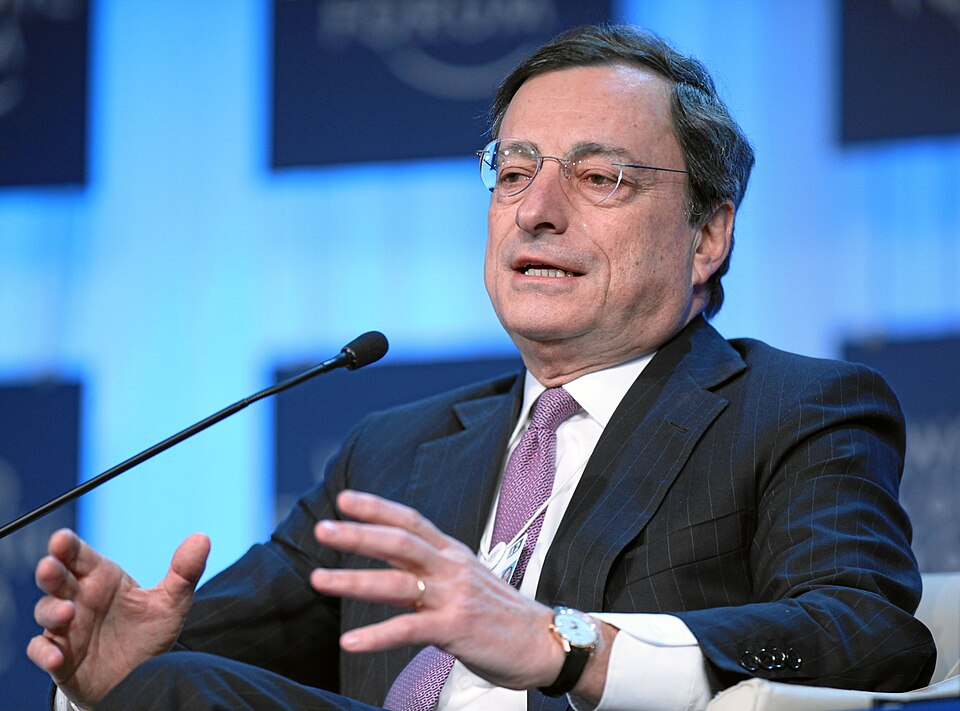
\includegraphics[width=\linewidth]{figures/lecture-09/draghi-2012-wef-davos.jpg}
\end{column}
\begin{column}{0.44\textwidth}
\Large\raggedright
``Within our mandate, the ECB is ready to do \textbf{\color{pelAccent}whatever it takes} to preserve the euro. And believe me, it will be enough.''
\vspace{0.3cm}

\normalsize Mario Draghi, ECB President\\
Global Investment Conference, London, \textbf{26 July 2012}
\end{column}
\end{columns}
\vspace{0.2cm}
\pelTableNote{Quote: ECB, verbatim of the remarks. Photo: Draghi at the World Economic Forum, Davos, 27 January 2012 (not the London conference). World Economic Forum, swiss-image.ch, photo by Monika Flueckiger, CC BY-SA 2.0, via Wikimedia Commons.}
\end{frame}

\begin{frame}{Normal times: one lever}
\begin{columns}[c]
\begin{column}{0.48\textwidth}
\footnotesize
\bi
  \item The ECB sets the price of money for \textbf{banks}: what they earn parking money at the ECB (\textbf{deposit facility}), what they pay to borrow from it
  \item No bank lends to another for less than the deposit rate: market rates sit on this floor
  \item Banks pass it on to firms and households
\ei
\vspace{0.1cm}
This is Monday's LM: the ECB picks $\bar i$
\end{column}
\begin{column}{0.48\textwidth}
\centering
\begin{tikzpicture}[x=0.8cm,y=0.75cm]
  \draw[pelBorder, line width=1pt] (0,0) -- (0,4.2);
  \draw[very thick, pelDanger] (-0.2,3.6) -- (4.6,3.6) node[right, font=\scriptsize, align=left] {Marginal lending\\2.90\%};
  \draw[very thick, pelSlate] (-0.2,2.4) -- (4.6,2.4) node[right, font=\scriptsize, align=left] {Main refinancing\\2.65\%};
  \draw[very thick, pelAccent] (-0.2,1.2) -- (4.6,1.2) node[right, font=\scriptsize, align=left] {\textbf{Deposit facility}\\\textbf{2.50\%}};
  \draw[thick, pelText, decorate] plot[smooth] coordinates {(0.2,1.35) (1.0,1.30) (1.8,1.38) (2.6,1.32) (3.4,1.36) (4.4,1.31)};
  \node[font=\scriptsize, pelText] at (2.3,0.75) {overnight market rate};
\end{tikzpicture}
\pelTableNote{Rates in force since 16 September 2026. Not to scale.}
\end{column}
\end{columns}
\end{frame}

\begin{frame}{When one lever is not enough: the unorthodox toolbox}
\scriptsize
\renewcommand{\arraystretch}{1.0}
\begin{tabular}{L{3.0cm}L{6.4cm}L{3.6cm}}
\toprule
\textbf{Tool} & \textbf{In plain words} & \textbf{When} \\
\midrule
\textbf{A promise}: Outright Monetary Transactions & Buy, with no preset limit, the bonds of a country under market attack, if it accepts a rescue programme & Sept 2012. Never activated \\
\textbf{Negative rates} & Banks \emph{pay} to park money at the ECB, to push them to lend & June 2014 to July 2022; lowest $-0.50\%$ \\
\textbf{Asset purchases} (``QE'') & The ECB buys bonds with new money: long-term rates fall when short rates cannot & APP 2015 (EUR 60 bn/month); PEPP 2020 (EUR 750 bn) \\
\textbf{Long-term loans to banks} & Cheap funding for several years, linked to lending to firms and households & In the low-rate years \\
\textbf{Forward guidance} & Say where rates are heading, to move expectations today & In the low-rate years \\
\textbf{Transmission Protection Instrument} & Buy a country's bonds if spreads widen in a disorderly way, unjustified by fundamentals & Created 2022. Never activated \\
\bottomrule
\end{tabular}
\pelTableNote{Sources: ECB press releases (6 Sept 2012, 22 Jan 2015, 18 Mar 2020); ECB key interest rates; ECB strategy statement 2025; ECB report on monetary policy tools (OMT and TPI never activated).}
\end{frame}

\begin{frame}{Unorthodox: a choice, with costs}
\footnotesize
\bi
  \item Each tool answered a crisis: the euro crisis (2012), inflation stuck too low (2014--15), the pandemic (2020), bond market stress as rates rose (2022)
  \item The 2025 strategy keeps them all, for use near the lower bound or when transmission is impaired. Today rates are the main tool again, and the APP and PEPP portfolios shrink as bonds mature
  \item The costs are debated:
  \bi
    \item side effects: bank profits under negative rates, higher asset prices, a huge central bank balance sheet
    \item legal limits: buying government bonds comes close to financing governments, which the Treaty forbids; OMT was challenged in court
  \ei
\ei
\vspace{0.1cm}
\begin{block}{An evaluation puzzle}
OMT was never used, yet it is credited with calming markets. How do you estimate the effect of a \textbf{promise}? Hint: Part I, event studies around the announcement dates
\end{block}
\end{frame}

\begin{frame}{The deposit facility rate, 2022--2026: Monday's $\bar i$}
\centering
\begin{tikzpicture}
\begin{axis}[pel chart, width=0.9\textwidth, height=0.6\textheight,
    xmin=2022.4, xmax=2027.0, ymin=0, ymax=4.6,
    xtick={2023,2024,2025,2026}, xticklabel style={/pgf/number format/1000 sep=},
    ylabel={\%}, ytick={0,1,2,3,4}]
  \addplot[const plot, very thick, pelAccent] coordinates {(2022.40,0.00) (2022.567,0.00) (2022.701,0.75) (2022.836,1.50) (2022.970,2.00) (2023.104,2.50) (2023.219,3.00) (2023.353,3.25) (2023.468,3.50) (2023.584,3.75) (2023.718,4.00) (2024.447,3.75) (2024.715,3.50) (2024.811,3.25) (2024.964,3.00) (2025.096,2.75) (2025.192,2.50) (2025.307,2.25) (2025.441,2.00) (2026.458,2.25) (2026.707,2.50) (2026.880,2.50)};
  \node[font=\scriptsize, pelText, anchor=south] at (axis cs:2023.72,4.05) {4.00 (Sept 2023)};
  \node[font=\scriptsize, pelText, anchor=north] at (axis cs:2025.9,1.95) {2.00 (June 2025)};
  \node[font=\scriptsize, pelAccent, anchor=south] at (axis cs:2026.6,2.55) {2.50 now};
\end{axis}
\end{tikzpicture}
\pelTableNote{Source: ECB, Key ECB interest rates (dates with effect from). Not shown: until July 2022 the rate was negative ($-0.50\%$).}
\end{frame}

\begin{frame}{The 2025 strategy assessment}
\small
The ECB reviews its strategy periodically. The 2025 statement confirms 2\%, symmetry and the medium term, and draws lessons from the low-inflation period and the post-pandemic inflation surge:
\bi
  \item The environment will stay uncertain, ``with larger target deviations in \textbf{both} directions'' (geopolitics, AI, demography, climate)
  \item Large, sustained deviations call for ``\textbf{appropriately forceful or persistent}'' action, in either direction
  \item Decisions rest on the most likely path \textbf{and} the risks around it: scenario and sensitivity analysis
  \item Financial stability is ``a precondition for price stability''
\ei
\vspace{0.1cm}
Next assessment: \textbf{2030}
\pelTableNote{ECB monetary policy strategy statement (2025), paras 1, 6, 9, 12.}
\end{frame}

\begin{frame}{The latest decisions}
\scriptsize
\begin{columns}[T]
\begin{column}{0.48\textwidth}
\textbf{10 September 2026: +25 basis points}
\bi
  \item Deposit rate to 2.50\% (from 16 September)
  \item The Middle East conflict keeps inflation ``well above target for an extended period''
  \item Staff projections, inflation: 3.0\% (2026), 2.5\% (2027), 2.1\% (2028)
  \item Growth: 0.9\%, 1.4\%, 1.5\%
\ei
\end{column}
\begin{column}{0.48\textwidth}
\textbf{29 October 2026: unchanged}
\bi
  \item Inflation 3.8\% in September; energy inflation 18.9\%
  \item Underlying inflation broadly stable, wages moderate; unemployment 6.4\%
  \item Energy shock: upside risk to inflation, downside risk to growth
  \item ``Data-dependent and meeting-by-meeting''; no pre-commitment
\ei
\end{column}
\end{columns}
\vspace{0.15cm}
\begin{block}{}
A supply shock pushes prices up and output down: the central bank cannot fix both with one rate
\end{block}
\pelTableNote{ECB, Monetary policy decisions, 10 September 2026; Combined monetary policy decisions and statement, 29 October 2026. Rates also rose in June 2026 (to 2.25\%, from 17 June).}
\end{frame}

\begin{frame}{What the ECB says to governments}
\footnotesize
From the 29 October statement:
\begin{block}{}
\footnotesize ``Fiscal sustainability is a crucial anchor for broader economic stability. Fiscal responses to the energy shock should be \textbf{temporary, targeted and tailored}.''
\end{block}
\vspace{0.1cm}
From the \textbf{Financial Stability Review}, published yesterday (18 November):
\bi
  \item In the euro area, ``elevated debt levels, growing sovereign borrowing needs'' and more leveraged investors increase the risk of ``abrupt repricing'' of government bonds
  \item Higher energy prices and weak growth ``could further strain public finances, allowing governments less room to respond to shocks''
\ei
\vspace{0.05cm}
\textbf{For discussion}: the escape clause opens room for energy spending; the ECB asks that it be temporary and targeted. Who checks that it is?
\pelTableNote{ECB, Combined monetary policy decisions and statement, 29 October 2026; ECB press release on the Financial Stability Review, 18 November 2026.}
\end{frame}

\begin{frame}{How a rate rise reaches firms: through banks}
\small
In the euro area banks provide most of the credit, so the banking channel matters (Lane, 2023):
\vspace{0.1cm}

\centering\footnotesize
\begin{tabular}{L{3.2cm}L{9.4cm}}
\toprule
\textbf{Channel} & \textbf{Mechanism}\\
\midrule
Cost of capital & Banks pass the policy rate on to lending rates: borrowing costs more \\
Balance sheet & Asset prices and collateral fall: borrowers' net worth falls, credit gets dearer \\
Bank lending & Banks' own funding costs rise and liquidity falls: they supply fewer loans \\
Risk taking & With higher rates, banks take less risk: credit supply contracts \\
\bottomrule
\end{tabular}
\vspace{0.15cm}

\raggedright\small
Monday's IS-LM has only the first channel. The others are why the size and speed of the effect must be \textbf{measured}, not assumed
\pelTableNote{Lane, P. R., ``The banking channel of monetary policy tightening in the euro area'', speech at the NBER Summer Institute, 12 July 2023.}
\end{frame}

%=============================================================================
\section{What it means for evaluation}
%=============================================================================

\begin{frame}{Reading 2026 with Monday's model}
\begin{columns}[c]
\begin{column}{0.5\textwidth}
\small
\bi
  \item ECB: rates up (LM up), against inflation from the energy shock
  \item Governments: more defence and energy spending (IS right), under escape clauses
  \item A policy mix in \textbf{opposite} directions
\ei
\vspace{0.1cm}
\footnotesize
Limits: IS-LM takes prices as given, but this is an \textbf{inflation} story; and it ignores debt and expectations. A first map, not the answer
\end{column}
\begin{column}{0.47\textwidth}
\centering
\begin{tikzpicture}[scale=0.85]
  \draw[-{Stealth[length=2.2mm]}, thick] (0,0) -- (5.6,0) node[below left, font=\footnotesize] {Output, $Y$};
  \draw[-{Stealth[length=2.2mm]}, thick] (0,0) -- (0,4.6) node[above right, font=\footnotesize] {$i$};
  \draw[very thick, pelSlate] (0.6,4.2) -- (4.4,0.4) node[right, font=\footnotesize] {IS};
  \draw[very thick, pelSlate, dashed] (1.4,4.2) -- (5.2,0.4) node[right, font=\footnotesize] {IS$'$};
  \draw[very thick, pelAccent] (0,1.6) node[left, font=\footnotesize] {$\bar i$} -- (5.3,1.6) node[right, font=\footnotesize] {LM};
  \draw[very thick, pelAccent, dashed] (0,2.4) node[left, font=\footnotesize] {$\bar i'$} -- (5.3,2.4) node[right, font=\footnotesize] {LM$'$};
  \fill (3.2,1.6) circle (2pt) node[below left, font=\footnotesize] {A};
  \fill[pelAccent] (3.2,2.4) circle (2pt) node[above right, font=\footnotesize] {A$'$};
\end{tikzpicture}
\pelTableNote{Drawn so that the two shifts offset on output. They need not.}
\end{column}
\end{columns}
\end{frame}

\begin{frame}{Three evaluation questions the documents leave open}
\small
\be
  \item \textbf{The reforms behind the 7 years}: the Council monitors whether steps are completed; the EFB calls the assessment ``cursory''. Did shorter bankruptcy proceedings, more childcare places\ldots\ change outcomes?
  \item \textbf{The energy measures}: ``targeted and cost-effective'' is an ex ante promise. What counterfactual would show it ex post?
  \item \textbf{Monetary policy}: the ECB raised rates in 2026. How much of the slowdown is due to rates and how much to the energy shock itself? The identification problem of Part I, at the scale of a continent
\ee
\vspace{0.15cm}
\begin{block}{}
\centering The rules and the ECB set the \textbf{envelope}. Evaluation asks what is done \textbf{inside} it, and whether it works
\end{block}
\end{frame}

\begin{frame}{For Friday's discussion}
\small
Groups of 2--3. Pick one:
\be
  \item You advise the Parliamentary Budget Office. Italy reports its energy measures to Brussels in April 2027. List three pieces of evidence you would ask for, beyond ``eligibility''
  \item The EFB says flexibility ``risks undermining the credibility'' of the rules. The government says it is needed for security. Write the strongest argument for each side in five lines
  \item The ECB raised rates while governments increased spending. Using IS-LM, explain what happens to output and to investment, and what the model cannot tell you
\ee
\end{frame}

\begin{frame}{Readings}
\footnotesize
\textbf{Core}
\bi
  \item European Fiscal Board, Annual Report 2025: Key messages and Executive summary
  \item ECB, An overview of the ECB's monetary policy strategy (2025)
  \item ECB, Combined monetary policy decisions and statement, 29 October 2026
\ei
\textbf{Documents used today} (on the site, Lectures page)
\bi
  \item Regulation (EU) 2024/1263, Council Regulation (EU) 2024/1264, Directive (EU) 2024/1265
  \item Council Recommendation endorsing Italy's plan (January 2025)
  \item Council Recommendation on Italy's national escape clause (November 2026)
  \item ECB strategy statement (2025); ECB press releases of 10 September and 18 November 2026
  \item Lane (2023), The banking channel of monetary policy tightening in the euro area
\ei
\textbf{Further}: Darvas, Welslau and Zettelmeyer (2024), Bruegel; Alesina and Passalacqua (2016); Kydland and Prescott, Nobel background note (2004)
\end{frame}

\pelQuestions

\end{document}
